% !TEX root =  ../report.tex
% !TeX spellcheck = en-GB

\section{Testing}
\label{s:test}
Throughout development, an example application that was previously developed using the OP2 API was used to test code generation, and verify the results. The application is called \textit{airfoil}, and it has been used for validating generated OP2 code before \cite{gpudesign}, as it makes use of all the key features including having both direct and indirect loops.
\par
\textit{airfoil} is a computational fluid dynamics application which models the air flow around an aeroplane wing, using unstructured grid to discretise the space. A document detailing the \textit{airfoil} code is available on the OP2 website \cite{airfoil}. Figure \ref{fig:airfoil_mesh} is an simple 120 x 60 mesh for \textit{airfoil}, showing the wing shape, and increasing granularity close to the shape. Each quadrilateral represents a cell.\par
\begin{figure}[h!]
  \centering
  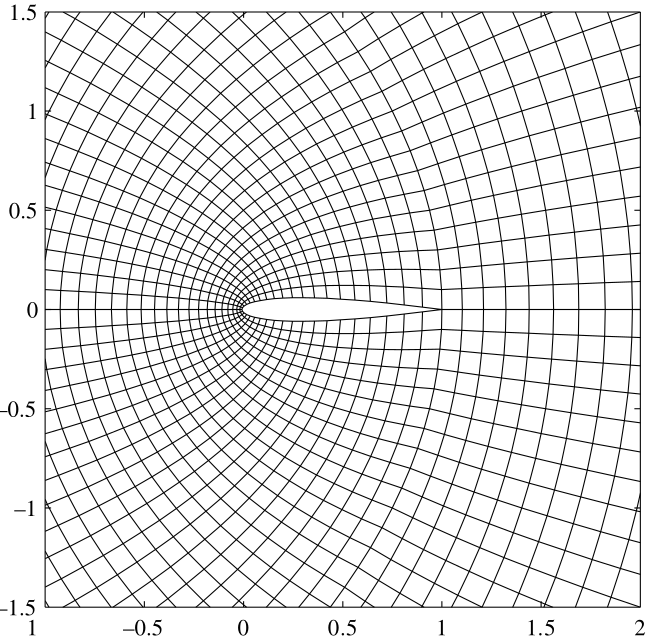
\includegraphics[width=.55\textwidth]{airfoil}
\caption{Rendering of an \textit{airfoil} mesh. Diagram from \cite{gpudesign}}
\label{fig:airfoil_mesh}
\end{figure}
\par
\vfill
\noindent To ensure that the test cases selected definitely validate the implementation, the requirements set out in the Specification must be revisited. They are summarised in the next Section.
\clearpage
\subsection{Requirements}
  \begin{outline}[enumerate]
  \1 Source code files must be produced as the output of the new code generation Python script.
  \1 The generated source code files must be valid.
  \2 C code must compile using \verb|icc| without errors;
  \2 CUDA code must compile with \verb|nvcc| without errors.
  \1 The compiled executable must invoke a re-compilation stage, if the feature is enabled.
  \2 Re-compilation must also complete without error;
  \2 The binary must execute code that has been compiled during its execution.
  \1 Constant values from the input must be available to the User Function.
  \2 If JIT is enabled, they must be turned into \verb|#define| directives;
  \2 Otherwise they must be copied to device memory.
  \1 The compiled executable must produce a result within some tolerance of the expected result.
  \1 The OP2 API must not be modified.
  \end{outline}

\noindent Section \ref{ss:results} is the final results of the test plan used throughout the project whenever a work done needed to be validated. Each test  ensures that a requirement from the above list has been met, and also includes the date when it first passed.
\par
Requirement 6 can be trivially accepted when testing, since the implementation did not modify the OP2 API. There is no test for this requirement.

\subsection{Initial State}
\begin{wrapfigure}[18]{l}{0.45\textwidth}
  \centering
\caption{\textit{airfoil} folder initial state}
\label{fig:files_a}
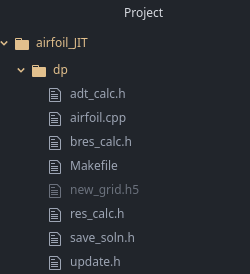
\includegraphics[width=0.4\textwidth]{files1}
\end{wrapfigure}
The initial state for testing is a folder containing the source files for \textit{airfoil}, as listed in Figure \ref{fig:files_a}. The Application File is \verb|airfoil.cpp|, and the five header files each contain a User Function for the parallel loop with the same name.
\par
\verb|new_grid.h5| is the name of the input data file, formatted in the Heterogeneous Data Format (HDF5) \cite{HDF5}. This file can be obtained from the OP2 website \cite{op-dsl}, and must be converted from \verb|.txt| to \verb|.h5| using the \verb|convert_mesh| tool.
\par
OP2 already provides a standard set of functions for performing file I/O on an HDF5 file, which \textit{airfoil} uses. The contents of the file can be viewed using the \verb|hdump| utility, which comes with an HDF5 installation.

\clearpage
\subsection{Test Plan \& Results}
\label{ss:results}

\hspace{\parindent}\minititle{``Source code files must be produced as the output of the new code generation Python script."}
To test the code generation, the python script \verb|op2.py| is called in the directory, passing the main application file \verb|airfoil.cpp| as an argument, as well as the string \verb|JIT| to make sure the correct GPU code generation script is used. \par
The environmental variable \verb|$OP2_INSTALL_PATH| can be assumed to hold to full path to the \verb|op2/| folder in the top level of the OP2 repository. Since the translation script is in a sub-directory of \verb|translator/|, which is also a top-level folder, the path to the Python translator script will be as shown below.
\codeline{> python2 \$OP2_INSTALL_PATH/../translator/c/python/op2.py airfoil.cpp JIT}{}

\noindent After running this command in the \textit{airfoil} directory, the expected outcome is that a new file: \verb|airfoil_op.cpp| is created, as well as a new directory named \verb|cuda/|, which will contain with eleven CUDA source code files it: two kernel files for each of the five parallel loops, and a single Central Kernels File, named \verb|airfoil_kernels.cu|.
\par
This test is considered a pass if these files exist, as their contents will be validated as correct if the following tests pass. A folder called \verb|seq/| is also created by the translator script \verb|translator/c/python/jit/op2_gen_seq_jit.py|, which was not completed as part of this project, but part of the \verb|feature/lazy-execution| branch.
\par
If the environmental variable \verb|OP_AUTO_SOA| is set to one, the code will be generated with transformations to automatically use the Struct-of-Arrays data structures, overwriting any generated source files that exist already. To confirm the functionality is working with both, the generated files need to be deleted, and the script invoked again once the environmental variable has been set.

\begin{wrapfigure}[13]{l}{0.45\textwidth}
\caption{\textit{airfoil} folder after Code Generation}
\label{fig:files_b}
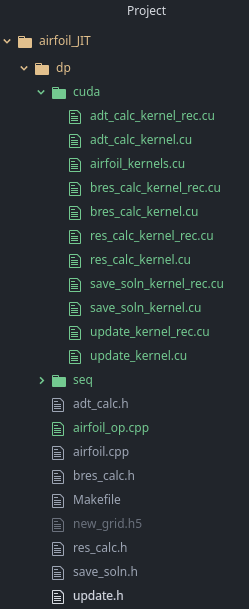
\includegraphics[width=0.4\textwidth]{files2}
\end{wrapfigure}
\par
Figure \ref{fig:files_b} shows the folder after a passing test case of running the OP2 translation script. The folder appears identical whether automatic\\ Struct-of-Arrays transformation is enabled or not, which is the expected outcome, so the Figure has not been duplicated.\par
When compared to Figure \ref{fig:files_a}, all the additional files have been generated by the code generation script. As expected, there are two kernel files for each parallel loop, and a single Central Kernels File in the \verb|cuda/| directory, and a Modified Application file in the root.
\par

\testresult{pass}{03/12/2019}

\minititle{``The generated source code files must be valid."}
The validity of the generated source code files will be confirmed by the initial compilation of the binary completing without error, both when JIT compilation is enabled and disabled. Recall that even with JIT compilation enabled, the AOT compiler is still required to produce an initial binary. If any errors are produced by the compiler, the code generated is not valid, and therefore is of no further use.
\par
In the \verb|airfoil_JIT| folder, compilation is done using the Makefile, and for the initial compilation of the binary, the target is \verb|airfoil_cuda|. The Makefile produces a binary with JIT compilation enabled by default, so the command to compile it will be: \\\verb|make airfoil_cuda|
\par Whereas, to produce a binary that will execute only Ahead-Of-Time compiled code, the command will be: \\\verb|make airfoil_cuda JIT=FALSE|
\par \noindent The resulting command executed by the Makefile is: \vspace{-1em}
\begin{verbatim}
nvcc -gencode arch=compute_60,code=sm_60 -m64 -Xptxas=-v
   --use_fast_math -O3 -lineinfo [-DOP2_JIT]
   -I$OP2_INSTALL_PATH/c/include
   -I$HDF5_INSTALL_PATH/include -Icuda -I.
   -c -o cuda/airfoil_kernels_cu.o cuda/airfoil_kernels.cu
\end{verbatim}
The inclusion of \verb|-DOP2_JIT| depends on which of the two above commands was called. Both commands will need to be tested for errors when the code base has been generated both with and without automatic Struct-of-Arrays transformations, giving four test cases. The generated code will also need to be manually inspected to ensure that transformations have been made when \verb|OP_AUTO_SOA| is enabled.
\begin{wrapfigure}[18]{l}{0.45\textwidth}
\caption{\textit{airfoil} folder after Ahead-Of-Time compilation}
\label{fig:files_c}
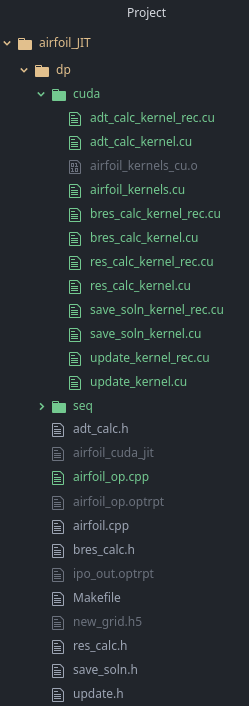
\includegraphics[width=0.4\textwidth]{files3}
\end{wrapfigure}
\par
\noindent Figure \ref{fig:files_c} shows the folder after the make command has been successfully executed. As before, the folder will appear almost identical for all four test cases, so the Figure has not been duplicated.\par
In the figure the first new file that can be seen is a single object file in the \verb|cuda/| folder, which is the result of compiling the Central Kernels File and all the kernels that are not marked \verb|_rec| into a single object binary.
\par  In the parent directory the executable \verb|airfoil_cuda_jit| has been generated, which statically links the above object file, so does not require access to it at run-time. If JIT compilation is not enabled, the binary is just called \verb|airfoil_cuda|.\par Lastly, a number of optimisation reports have been generated by the Intel C compiler.\par
\vspace{3cm}
\noindent The test results and dates for the four test cases are shown in a matrix below.
\begin{table}[h]
\centering
\renewcommand{\arraystretch}{1.5}
\begin{tabular}{| c || c | c |}
\hline
JIT & \verb|OP_AUTO_SOA=0| & \verb|OP_AUTO_SOA=1| \\
\hhline{|=|=|=|}
TRUE &\textbf{\textcolor{green!20!black}{PASSED}}. 16/01/2020 &\textbf{\textcolor{green!20!black}{PASSED}}. 17/01/2020 \\
\hline
FALSE&\textbf{\textcolor{green!20!black}{PASSED}}. 16/01/2020 &\textbf{\textcolor{green!20!black}{PASSED}}. 17/01/2020 \\
\hline
\end{tabular}
\end{table}

\minititle{``The compiled executable must invoke a re-compilation stage, if the feature is enabled."}
\label{sss:jit_comp}
For this test to be considered a pass, a compiler process must be started during the execution of the binary, and must complete without producing errors. As described previously, in Section \ref{sss:mkf}, there exists a check for success in the code, and the terminal output of the compilation is dumped to a file named \verb|jit_compile.log|.
\par
The executable printing the compilation duration to the console output like the example below confirms the compilation has completed, and success can be confirmed by checking the compiler log for errors. If none are found, requirement \textbf{3i} has been met: \textbf{``Re-compilation must also complete without error"}.

\begin{figure}[h!]
  \caption{\label{fig:jit_ex}Example success output}
\begin{verbatim}
> ./airfoil_cuda_jit
...
JIT compiling op_par_loops
  Completed: 5.588549s
\end{verbatim}
\end{figure}

\par\noindent
It should be the case that these lines are \textbf{not} printed if the executable was compiled with JIT compilation disabled, otherwise the part of the requirement that states \textbf{``\ldots, if the feature is enabled"} has been violated.\par
In order to determine whether sub-requirement \textbf{3ii} has been met: \textbf{``The binary must execute code that has been compiled during its execution"}, one of the Kernel files that will be compiled at runtime is manually edited to contain a print statement, or some other identifier to confirm which version is being executed: the run-time compiled or the original.\par
As with the second requirement there are 4 test cases. It is possible that the state of \verb|OP_AUTO_SOA| could interfere, so both enabled and disabled will need to be tested for both possible states for JIT compilation.
\clearpage
\begin{wrapfigure}[21]{l}{0.45\textwidth}
\caption{\textit{airfoil} folder after Just-In-Time Compilation}
\label{fig:files_d}
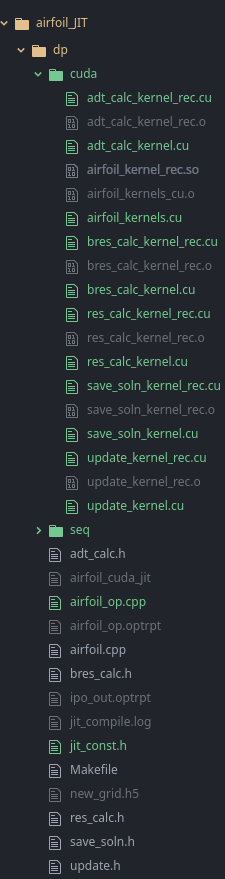
\includegraphics[width=0.4\textwidth]{files4}
\end{wrapfigure}
Figure \ref{fig:files_d} shows the \textit{airfoil} folder after the JIT compilation stage has completed successfully. In the Figure, there is now an object file for each of the parallel loops, as well as a new shared object in the \verb|cuda/| folder, which will have been loaded by the running executable. Some other files have also been generated, including the compilation log file \verb|jit_compile.log|, and the constants header file \verb|jit_const.h| which is part of the next requirement.
\par
The JIT compilation log file does not contain any errors, and the expected files have been generated, so the main part of the requirement has been met.
\par
Manually adding a print statement to only the re-compiled kernels confirms that the correct kernels are being executed, and JIT compilation is enabled, the executable is utilising functions that have been compiled as part of it's execution.
\begin{table}[b]
\raggedleft
\renewcommand{\arraystretch}{2.5}
\begin{tabular}{| c || c | c |}
\hline
JIT & \verb|OP_AUTO_SOA=0| & \verb|OP_AUTO_SOA=1| \\
\hhline{|=|=|=|}
TRUE & \shortstack{\textbf{\textcolor{green!20!black}{PASSED}}.\\22/01/2020} &\shortstack{\textbf{\textcolor{green!20!black}{PASSED}}.\\22/01/2020} \\
\hline
FALSE&\shortstack{\textbf{\textcolor{green!20!black}{PASSED}}.\\22/01/2020} &\shortstack{\textbf{\textcolor{green!20!black}{PASSED}}.\\22/01/2020} \\
\hline
\end{tabular}
\hspace{-0.5cm}
\end{table}

\minititle{``Constant values from the input must be available to the User Function."}
This test simply requires that the User Function is able to access the values of input constants when they are executing on the GPU. For Kernels compiled with JIT compilation disabled, this requires that they are copied to device memory, and for JIT enabled Kernels they must be defined literals.
\par
The \textit{airfoil} program includes a number of input constants, where six have a dimension of 1, and one has a dimension of 4 named \verb|qinf| - all holding values of the type \verb|double|. It never exercises the functionality of accessing \verb|qinf| using an expression however, so to test that this functionality works correctly, additional code needs to be added inside the User Function.
\par This can be solved at the same time as testing the other constants by adding to the code generation script, such that inside the User Function the values of constants are printed. This should include a loop over \verb|qinf| such that it is accessed using an index variable, and with literal values.

\begin{lstlisting}[backgroundcolor=\color{lightgray!20}, language=Python]
|IF('blockIdx.x == 0 && threadIdx.x == 0')
|for nc in range (0,len(consts)):
|  comm(consts[nc]['name'])
|  if consts[nc]['dim']==1:
|  code('printf("'+name+'-'+consts[nc]['name']+
        ': %1.17e\\n",'+ consts[nc]['name']+');')
|  else:
|    FOR('i','0',consts[nc]['dim'])
|    code('printf("'+name+'-'+consts[nc]['name']+
          '[%d]: %1.17e\\n", i,'+consts[nc]['name']+'[i]);')
|    ENDFOR()
|    for i in range (0,int(consts[nc]['dim'])):
|      code('printf("'+name+'-'+consts[nc]['name']+
            '['+str(i)+']: %1.17e\\n",'+ consts[nc]['name']+
            '['+str(i)+']);')
|ENDIF()
\end{lstlisting}
The above code is left in the translator script, at lines [259-281], but has been commented out as printing this much to the terminal is very detrimental to performance. It should not be included for benchmarking or production code generation.
\par
For \textit{airfoil}, the code added to the end of the JIT enabled \verb|save_soln| User Function is:
\begin{lstlisting}[backgroundcolor=\color{red!20},language=C]
|  if (blockIdx.x == 0 && threadIdx.x == 0) {
|    //gam
|    printf("save_soln-gam: %1.17e\n",gam);
|    //gm1
|    printf("save_soln-gm1: %1.17e\n",gm1);
|    //cfl
|    printf("save_soln-cfl: %1.17e\n",cfl);
|    //eps
|    printf("save_soln-eps: %1.17e\n",eps);
|    //mach
|    printf("save_soln-mach: %1.17e\n",mach);
|    //alpha
|    printf("save_soln-alpha: %1.17e\n",alpha);
|    //qinf
|    for (int i = 0; i < 4; ++i)
|    {
|      printf("save_soln-qinf_OP2CONSTANT[%d]: %1.17e\n", i,
               qinf_OP2CONSTANT[i]);
|    }
|    printf("save_soln-qinf_0_OP2CONSTANT: %1.17e\n",
             qinf_0_OP2CONSTANT);
|    printf("save_soln-qinf_1_OP2CONSTANT: %1.17e\n",
             qinf_1_OP2CONSTANT);
|    printf("save_soln-qinf_2_OP2CONSTANT: %1.17e\n",
             qinf_2_OP2CONSTANT);
|    printf("save_soln-qinf_3_OP2CONSTANT: %1.17e\n",
             qinf_3_OP2CONSTANT);
|  }
\end{lstlisting}
When the above lines are included, the expected output for each loop is that each one dimensional constant will be printed along with the function it is being used in. Then, the multi value constants will be printed twice: once using a variable \verb|i| to index it, and again using literal values.
\par
The generated code for an AOT kernel is similar, but with modified references to the constants, since constant references are managed using a string replacement on all places where they appear in the User Function.\par
\clearpage
\noindent When the \verb|save_soln| loop is executed, the terminal output with JIT compilation is enabled will be the following if the values are available and correct:
\begin{lstlisting}[frame=none]
save_soln-gam: 1.39999997615814209e+00
save_soln-gm1: 3.99999976158142090e-01
save_soln-cfl: 8.99999976158142090e-01
save_soln-eps: 5.00000007450580597e-02
save_soln-mach: 4.00000005960464478e-01
save_soln-alpha: 5.23598775598298830e-02
save_soln-qinf_OP2CONSTANT[0]: 1.00000000000000000e+00
save_soln-qinf_OP2CONSTANT[1]: 4.73286385670476317e-01
save_soln-qinf_OP2CONSTANT[2]: 0.00000000000000000e+00
save_soln-qinf_OP2CONSTANT[3]: 2.61200015044213218e+00
save_soln-qinf_0_OP2CONSTANT: 1.00000000000000000e+00
save_soln-qinf_1_OP2CONSTANT: 4.73286385670476317e-01
save_soln-qinf_2_OP2CONSTANT: 0.00000000000000000e+00
save_soln-qinf_3_OP2CONSTANT: 2.61200015044213218e+00
\end{lstlisting}

\noindent Furthermore, when an \textit{airfoil} binary with JIT compilation enabled is executed, the \verb|jit_const.h| file should contain the following statements. Values correspond with those above.
\begin{lstlisting}[backgroundcolor=\color{green!20}, language=C]
|#define gam 1.39999997615814209e+00
|#define gm1 3.99999976158142090e-01
|#define cfl 8.99999976158142090e-01
|#define eps 5.00000007450580597e-02
|#define mach 4.00000005960464478e-01
|#define alpha 5.23598775598298830e-02
|#define qinf_0_OP2CONSTANT 1.00000000000000000e+00
|#define qinf_1_OP2CONSTANT 4.73286385670476317e-01
|#define qinf_2_OP2CONSTANT 0.00000000000000000e+00
|#define qinf_3_OP2CONSTANT 2.61200015044213218e+00
\end{lstlisting}
\vfill
\noindent The test results and dates for the four test cases are shown in a matrix below.
\begin{table}[h]
\centering
\renewcommand{\arraystretch}{1.5}
\begin{tabular}{| c || c | c |}
\hline
JIT & \verb|OP_AUTO_SOA=0| & \verb|OP_AUTO_SOA=1| \\
\hhline{|=|=|=|}
TRUE &\textbf{\textcolor{green!20!black}{PASSED}}. 21/01/2020 &\textbf{\textcolor{green!20!black}{PASSED}}. 21/01/2020 \\
\hline
FALSE&\textbf{\textcolor{green!20!black}{PASSED}}. 21/01/2020 &\textbf{\textcolor{green!20!black}{PASSED}}. 21/01/2020 \\
\hline
\end{tabular}
\end{table}
\clearpage
\minititle{``The compiled executable must produce a result within some tolerance of the expected result."}
The final test is that the result of the execution is within tolerance of the expected result. This test confirms that the contents of the file are not just valid but also correct.

\tinytitle{Expected Result}
The \textit{airfoil} OP2 application prints the value of the \verb|rms| (root mean square) variable every 100 iterations. According to the documentation, the first 1000 iterations for double precision should be exactly:\\
\begin{table}[h!]
\vspace{-2em}
\centering
\renewcommand{\arraystretch}{1.2}
\begin{tabular}{c c || c }
& & \verb|rms| \\
\hline
\multirow{10}{*}{Iterations} & 100 & $ 5.02186\times10^{-4} $ \\
& 200 & $ 3.41746\times10^{-4} $ \\
& 300 & $ 2.63430\times10^{-4} $ \\
& 400 & $ 2.16288\times10^{-4} $ \\
& 500 & $ 1.84659\times10^{-4} $ \\
& 600 & $ 1.60866\times10^{-4} $ \\
& 700 & $ 1.42253\times10^{-4} $ \\
& 800 & $ 1.27627\times10^{-4} $ \\
& 900 & $ 1.15810\times10^{-4} $ \\
& 1000 & $ 1.06011\times10^{-4} $
\end{tabular}
\caption{Expected values of rms}
\label{tab:expected}

\end{table}

\noindent The application code also includes a test of the result after 1000 iterations, which compares against the expected outcome and prints the calculated percentage difference using the equation:
\[\%diff = \abs{ (100 \times \frac{rms}{0.0001060114637578}) - 100 }\]
A difference of less than 0.00001\% is considered within tolerance due to the potential for minor floating point errors.
\clearpage
\tinytitle{Actual Results}

\noindent The tables below show the results output by the compiled binary every 100 iterations.
\begin{table}[H]
\renewcommand{\arraystretch}{1.2}
\caption{Console Output when JIT compilation is Enabled}
\label{tab:output}
\begin{tabular}{c c || c | c }
&  & \verb|OP_AUTO_SOA=0| & \verb|OP_AUTO_SOA=1| \\
\hline
\multirow{10}{*}{Iterations} & 100  & $ 5.02186\times10^{-4} $ & $ 5.02186\times10^{-4} $  \\
& 200  & $ 3.41746\times10^{-4} $ & $ 3.41746\times10^{-4} $  \\
& 300  & $ 2.63430\times10^{-4} $ & $ 2.63430\times10^{-4} $  \\
& 400  & $ 2.16288\times10^{-4} $ & $ 2.16288\times10^{-4} $  \\
& 500  & $ 1.84659\times10^{-4} $ & $ 1.84659\times10^{-4} $  \\
& 600  & $ 1.60866\times10^{-4} $ & $ 1.60866\times10^{-4} $  \\
& 700  & $ 1.42253\times10^{-4} $ & $ 1.42253\times10^{-4} $  \\
& 800  & $ 1.27627\times10^{-4} $ & $ 1.27627\times10^{-4} $  \\
& 900  & $ 1.15810\times10^{-4} $ & $ 1.15810\times10^{-4} $  \\
& 1000  & $ 1.06011\times10^{-4} $ & $ 1.06011\times10^{-4} $  \\
\hline
&&&\\
Accuracy & & $2.484679129111100\times10^{-11} \%$ & $2.489120021209601\times10^{-11} \%$ \\
&&&\\
\hline
\end{tabular}
\newline
\newline
\caption{Console Output when JIT compilation is Disabled}
\label{tab:output}
\begin{tabular}{c c || c | c }
&  & \verb|OP_AUTO_SOA=0| & \verb|OP_AUTO_SOA=1| \\
\hline
\multirow{10}{*}{Iterations} & 100  & $ 5.02186\times10^{-4} $ & $ 5.02186\times10^{-4} $  \\
& 200  & $ 3.41746\times10^{-4} $ & $ 3.41746\times10^{-4} $  \\
& 300  & $ 2.63430\times10^{-4} $ & $ 2.63430\times10^{-4} $  \\
& 400  & $ 2.16288\times10^{-4} $ & $ 2.16288\times10^{-4} $  \\
& 500  & $ 1.84659\times10^{-4} $ & $ 1.84659\times10^{-4} $  \\
& 600  & $ 1.60866\times10^{-4} $ & $ 1.60866\times10^{-4} $  \\
& 700  & $ 1.42253\times10^{-4} $ & $ 1.42253\times10^{-4} $  \\
& 800  & $ 1.27627\times10^{-4} $ & $ 1.27627\times10^{-4} $  \\
& 900  & $ 1.15810\times10^{-4} $ & $ 1.15810\times10^{-4} $  \\
& 1000  & $ 1.06011\times10^{-4} $ & $ 1.06011\times10^{-4} $  \\
\hline
&&&\\
Accuracy & & $2.486899575160351\times10^{-11} \%$ & $2.493560913308102\times10^{-11} \%$ \\
&&&\\
\hline
\end{tabular}
\end{table}
\vspace{-1.5em}
\noindent All of these results are well within tolerance. The requirement has been met.

\subsection{Benchmarking}
The functionality has now been confirmed to work as intended, and the technical requirements of the project have all been met: new code is able to be generated by the OP2 translator script, which can be compiled into a binary that will execute code it has compiled itself as part of it's execution. What remains is to benchmark the run-time of the application with JIT compilation enabled and disabled, and determine if there is any performance gain.
\par
The following results should be considered a benchmark of the Constant Definition optimisation, rather than JIT compilation as a whole, as further assertions at run-time are possible and could make even more use of the compiler being aware of the input data.

\subsubsection{Hardware}
Testing was done on a personal computer with an NVIDIA GeForce MX250 Graphics Card \cite{mx250} - and while this is able to execute the CUDA code and ensure it produces the right output, it is not sufficient to gather representative benchmarking data for the runtime of the \textit{airfoil} application. Using a personal computer system may result in noisy data, for example from the Operating System scheduling other tasks.
\par
In order to gather better data, access to a HPC cluster located in Cambridge, part of the Cambridge Service for Data-Driven Discovery (CSD3) \cite{csd3}, was approved - with the caveat that workloads for this project would be placed in a low priority queue.
\par
The supercomputer named \textit{Wilkes2} was used, which is the largest GPU enabled supercomputer for academic research in the UK. \textit{Wilkes2} has 90 nodes, each with the specifications in Table \ref{tab:wilkes2} \cite{wilkes2}. \clearpage

\begin{table}[h]
  \centering
  \renewcommand{\arraystretch}{1.5}
  \caption{\textit{Wilkes2} hardware specification}
  \label{tab:wilkes2}
\begin{tabular}{c |r l c}
CPU & 1 x&12-core Intel Xeon E5-2650 v4 2.2GHz & \cite{xeon}\\
RAM & &96GB &\\
GPU & 4 x&NVidia P100 16GB &\cite{p100}\\
\end{tabular}
\end{table}

\noindent The translator currently only generates code for a single graphics card, so only one of the four will be used. A possible extension would be to include MPI and divide the workload across multiple GPUs.

\subsubsection{Benchmarking Strategy}
The \textit{airfoil} program was also used for benchmarking, as it is reasonably representative of production applications. The input mesh remains the same size as in the previous Section where it was used for testing functionality, with 721,801 nodes, but the number of time step iterations was upped from 1000 to 1,000,000 to make any differences in run-time more noticeable. OP2's internal timing functions are used to sum the total time spent in each of the parallel loops, which can be compared between the versions with JIT compilation enabled and disabled.
\par
As discussed in Section \ref{sss:jit_comp} (Just-In-Time Compilation), the time taken for the invocation of the compiler at run-time to complete is also recorded, and will be included in the data. It is a one-time cost at the start of execution, but still needs to be considered.
% \par
% Given more time other OP2 applications would also have been used to compare data, however, finding a suitable HPC system and gaining access took a larger portion of the project's duration than expected.
\clearpage
\subsubsection{Results}
The graph in Figure \ref{fig:res_total} shows the mean total run-time of the four different configurations, averaged from five executions, in an attempt to further reduce any noise from factors other than those being tested. The percentage speed-up from the original version (blue) to JIT compiled (green) is shown above each pair of bars.

\begin{figure}[h!]
\begin{center}
\caption{Total Execution Time}
\label{fig:res_total}
\pgfplotsset{width=.6\linewidth,compat=1.8}
\begin{tikzpicture}
\begin{axis}[
  ybar,
  ymin=1000,
  ymax=2500,
  bar width=.6cm,
  enlargelimits=0.05,
  enlarge x limits={abs{0.5}},
  legend style={at={(1,0.95)},
    anchor=north},
  ylabel={Execution Time/s},
  symbolic x coords={Total},
  xtick=data,
  nodes near coords={},
  every node near coord/.append style={yshift=5pt}
  ]
  \addplot+[blue, fill=blue!20, name nodes near coords=AOTAOS]
  coordinates {(Total,2379.0361)};
  \addplot+[green!50!black,fill=green!20, name nodes near coords=JITAOS]
  coordinates {(Total,2378.349309)};
  \addplot+[blue, pattern=custom north west lines, hatchspread=1em, hatchcolor=blue!20, name nodes near coords=AOTSOA]
  coordinates {(Total,1910.25154)};
  \addplot+[green!50!black, pattern=custom north west lines, hatchspread=1em, hatchcolor=green!60, name nodes near coords=JITSOA]
  coordinates {(Total,1912.105723)};
\legend{JIT Disabled AoS,JIT Enabled AoS,JIT Disabled SoA,JIT Enabled SoA}
\end{axis}
\path (AOTAOS0) -- (JITAOS0) node[midway] (A) {0.03\%};
\path (AOTSOA0) -- (JITSOA0) node[midway] (A) {-0.1\%};
\end{tikzpicture}
\end{center}
\vspace{-1cm}
\end{figure}

\noindent The speed-up percentages above the bars were calculated using the formula below:
\[ \%speedup = \frac{\text{Initial Time}-\text{New Time}}{\text{Initial Time}} \times 100\%\]
Therefore a positive value indicates that the JIT compiled version completed faster, while a negative value indicates it was outperformed by the original.

\tinytitle{Analysis}

\noindent In Figure \ref{fig:res_total}, the speed-up for Array-of-Structs data layout is 0.03\%, which is only a very small improvement coming to about 1 second saved out of nearly 40 minutes. However the setup cost of run-time compilation is an average of 4.13 seconds, compared to essentially zero seconds to copy constants to device memory (0.0001s for all \textit{airfoil} constants). This duration does not vary significantly when either the size of the mesh or the number of iterations is increased.
\par
If the re-compilation time is excluded, the speed-up is 0.2\% for the actual execution of the application. From this, and the fact that compilation time is O(1) for input size, it follows that the speed-up could increase linearly with problem size, albeit at a shallow gradient. There will always be a constant initial cost, but every single iteration will complete fractionally faster. More iterations means more time saved.
\par
Unfortunately, when \verb|OP_AUTO_SOA=1| the object difference is that the executable with JIT compilation enabled is 0.1\% slower. As before, it should be considered that JIT compilation incurs a larger one-time cost at the start, and comparing just the application execution the runtime is 0.14\% faster. It would seem there is benefit possible for the SOA enabled build, but the problem size needs to be even greater for the per-iteration time reduction to outweigh the upfront cost, and the total execution time to be reduced.\par
\subsubsection{Results by Parallel Loop}
The runtime can be broken down into how long the application spent executing each of the parallel loops, and what speed-up each loop was able to see when applying JIT compilation. In the chart on the next page (Figure \ref{fig:res_func}), the speed-up of each parallel loop is plotted. Once again, a percentage is given above each pair of bars, which is the speed-up of the JIT compiled version compared to the version with JIT compilation disabled.
\par
As in Figure \ref{fig:res_total}, a positive value indicates that the JIT compilation enabled version completed faster, while a negative percentage means the version without JIT compilation had the shorter runtime.
\clearpage
\begin{figure}[ht]
\begin{center}
\caption{Execution Time by Function}
\label{fig:res_func}

\pgfplotsset{width=1.1\linewidth,compat=1.8}
\makebox[\textwidth][c]{
\begin{tikzpicture}
\begin{axis}[
  ybar,
  bar width=.5cm,
  enlargelimits=0.01,
  ymin=0,
  ymax=1400,
  enlarge x limits={abs{0.1}},
  legend style={at={(.05,.95)},
    anchor=north west},
  ylabel={Execution Time/s},
  symbolic x coords={setup,save\_soln,adt\_calc,res\_calc,bres\_calc,update},
  xtick=data,
  x tick label style={rotate=45,anchor=east},
  nodes near coords={},
  every node near coord/.append style={yshift=5pt}
  ]
  \addplot+[blue, fill=blue!20, name nodes near coords=AOTAOS]
  coordinates
  {(setup,0) (save\_soln,149.6223833) (adt\_calc,242.9445833) (res\_calc,1324.230383) (bres\_calc,25.66483333) (update,636.5739167)};
  \addplot+[green!50!black,fill=green!20, name nodes near coords=JITAOS]
  coordinates
  {(setup,4.125742667) (save\_soln,148.9582667) (adt\_calc,240.1570667) (res\_calc,1324.5283) (bres\_calc,25.20193333) (update,635.378)};
  \addplot+[blue, pattern=custom north west lines, hatchspread=1em, hatchcolor=blue!20, name nodes near coords=AOTSOA]
  coordinates
  {(setup,0) (save\_soln,99.07338) (adt\_calc,239.80552) (res\_calc,1028.33054) (bres\_calc,29.6906) (update,513.3515)};
  \addplot+[green!50!black, pattern=custom north west lines, hatchspread=1em, hatchcolor=green!60, name nodes near coords=JITSOA]
  coordinates
  {(setup,3.993373) (save\_soln,98.793325) (adt\_calc,238.07195) (res\_calc,1027.164025) (bres\_calc,29.023825) (update,515.059225)};

\legend{JIT Disabled AoS,JIT Enabled AoS,JIT Disabled SoA,JIT Enabled SoA}
\end{axis}
\path (AOTAOS0) -- (JITAOS0) node[midway] (A) {\small N/A};
\path (AOTSOA0) -- (JITSOA0) node[midway] (A) {\small N/A};

\path (AOTAOS1) -- (JITAOS1) node[midway] (A) {\small 0.44\%};
\path (AOTSOA1) -- (JITSOA1) node[midway] (A) {\small 0.28\%};

\path (AOTAOS2) -- (JITAOS2) node[midway] (A) {\small 1.15\%};
\path (AOTSOA2) -- (JITSOA2) node[midway] (A) {\small 0.72\%};

\path (AOTAOS3) -- (JITAOS3) node[midway] (A) {\small -0.02\%};
\path (AOTSOA3) -- (JITSOA3) node[midway] (A) {\small 0.11\%};

\path (AOTAOS4) -- (JITAOS4) node[midway] (A) {\small 1.80\%};
\path (AOTSOA4) -- (JITSOA4) node[midway] (A) {\small 2.25\%};

\path (AOTAOS5) -- (JITAOS5) node[midway] (A) {\small 0.19\%};
\path (AOTSOA5) -- (JITSOA5) node[midway] (A) {\small -0.33\%};
\end{tikzpicture}
}
\end{center}
\end{figure}
\vspace{-1cm}
\noindent The speed-up of the setup stage is marked Not Applicable (instead of negative four million percent) since the time taken to copy constants to device memory for \textit{airfoil} is essentially zero seconds.

\tinytitle{Analysis}

\noindent As with most HPC applications, different loops in \textit{airfoil} take up different proportions of the runtime. In Figure \ref{fig:res_func} it is clear that \textit{res\_calc} dominates the runtime, and is also the least able to benefit from the Constant Definition optimisation made in the JIT compiled code, since it was actually marginally slower for AoS. Looking into the source code, the loop body only uses the input constants three times: \verb|gm1| twice in quick succession, so would likely still be cached in the AOT compiled version; then \verb|eps| once a few lines later.
\par
Comparing this to \textit{bres\_calc}, which was the best affected by Constant Definition, the pattern holds as this function makes sixteen references to \verb|qinf|, as well as using \verb|gm1| twice. Although this could not be tested in the time available, it would seem logical that if the function that dominates the runtime is also making heavy use of input constants, the overall benefit to the application could be greater.
\par
\subsubsection{Results Conclusion}
What the results demonstrate most of all, is that there is definitely potential in Just in Time compilation. At one million time steps, the optimisation of Constant Definition was able to approximately make up the cost of re-compilation through fractional reduction in the time taken to perform every iteration, and increasing the problem size would only improve the speed-up.
\par
Since the assertion being made is only that values declared constant will remain constant, the time available for optimisation is only the time taken to read constant values from memory, which will not usually make up a significant proportion of the run-time.
\par
If more optimisations are implemented, which make further use of the inputs being known, and the per-iteration speed-up is increased, then the required problem size to see benefit will shrink, and the technique becomes even more valuable.
\par
Even without further optimisations, a small improvement to a very large solver application, which might be executing many millions of time-step iterations, can quickly outweigh the relatively tiny one-time cost of recompilation, and start to make an improvement to the overall runtime.
